\section*{РЕФЕРАТ}
\addcontentsline{toc}{section}{\protect РЕФЕРАТ}%
\paragraph*{Актуальность работы} В настоящее время ВВЭР-1000 является наиболее распространенным реактором в своей серии, а также достаточно продолжительно находится в эксплуатации. Со временем его срок службы был увеличен с 30 до 60 лет благодаря накопленным научным знаниям и анализу. Современная атомная энергетика имеет тренж на повышение мощности установок для обеспечения возрастающей энергетической потребности. Однако наличие ряда инвестиционных трудностей ограничивает в создании новых энергоблоков, соответственно необходимо делать упор на модернизацию и эксплуатацию существующих. Данная работа посвящена решению проблемы эксплуатации реактора ВВЭР-1000 в условиях повышения мощности, а также ее понижения при откллючении одного из трех и двух из трех ГЦН.
\paragraph*{Цель работы}
Цель состоит в исследовании температурных полей реакторной установки ВВЭР-1000 при работе на повышенной мощности, а также на пониженной при отключении одного из четырех и двух из четырех ГЦН.
\paragraph*{Основные задачи исследования}
\begin{itemize}
    \item Произвести теплофизический и нейтронно-физический расчет ВВЭР-1000 и определить характеристики РУ в номинальном режиме работы 
    \item Ознакомится с расчетной моделью программного комплекса ТРЕТОН и прозвести валидационный расчет РУ в номинальном режиме.
    \item Произвести рассчетное исследование работы реактора в режиме повышенной мощности, определить максимальные температуры и их превышения и сделать вывод о возможности работы реактора в таком режиме
    \item Произвести рассчетное исследование работы реактора при отключении одного из трех и двух из трех, произвести анализ температурных полей и сделать вывод о возможности работы РУ при пониженной мощности
\end{itemize}
\paragraph*{Практическая значимость} данной работы состоит в определении максимальных температур теплоносителя, оболочек и топлива для и выводов о работоспособности РУ в исследуемых режимах работы.
\subsection*{ОСНОВНОЕ СОДЕРЖАНИЕ РАБОТЫ}
\paragraph*{В главе 2} произведен теплофизический расчет термодинамических и гидравлическиъ параметров реакторной установки. Был расчитан КПД нетто термодинамического цикла $\eta_{\text{брутто}}=0.34$ и тепловая мощность $Q_{\text{теп}}=2.9 \cdot 10^3\ \text{МВт}$. Также было построено распределение температуры по высоте в наиболее нагруженном канале, которое представлено на \ref{pic:Tz-referat}. Была опрелена максимальная температура теплоносителя $T_{\text{ТН}^{\text{max}}} = 328.5\ ^\circ C$, запас до кипения теплоносителя составил $ 17.26\ ^\circ C$. Также была получена зависимость температуры внешней оболочки от высоте АЗ, максимальная температура составила $T_{\text{об}}^{\max} = 341.6 ^\circ C $, из чего сделан вывод об отсутствии пристеночного кипения. для  топлива максимальная температура составила $T_{\text{топ}} = 1559 ^\circ C$, что не превышает максимально допустимую температуру топилва при авариях. Также для исследуемой установки был расчитан КПД с учетом мощности на прокачку теплоносителя, который составил 0.342.
\begin{figure}[H]
	\begin{center}
		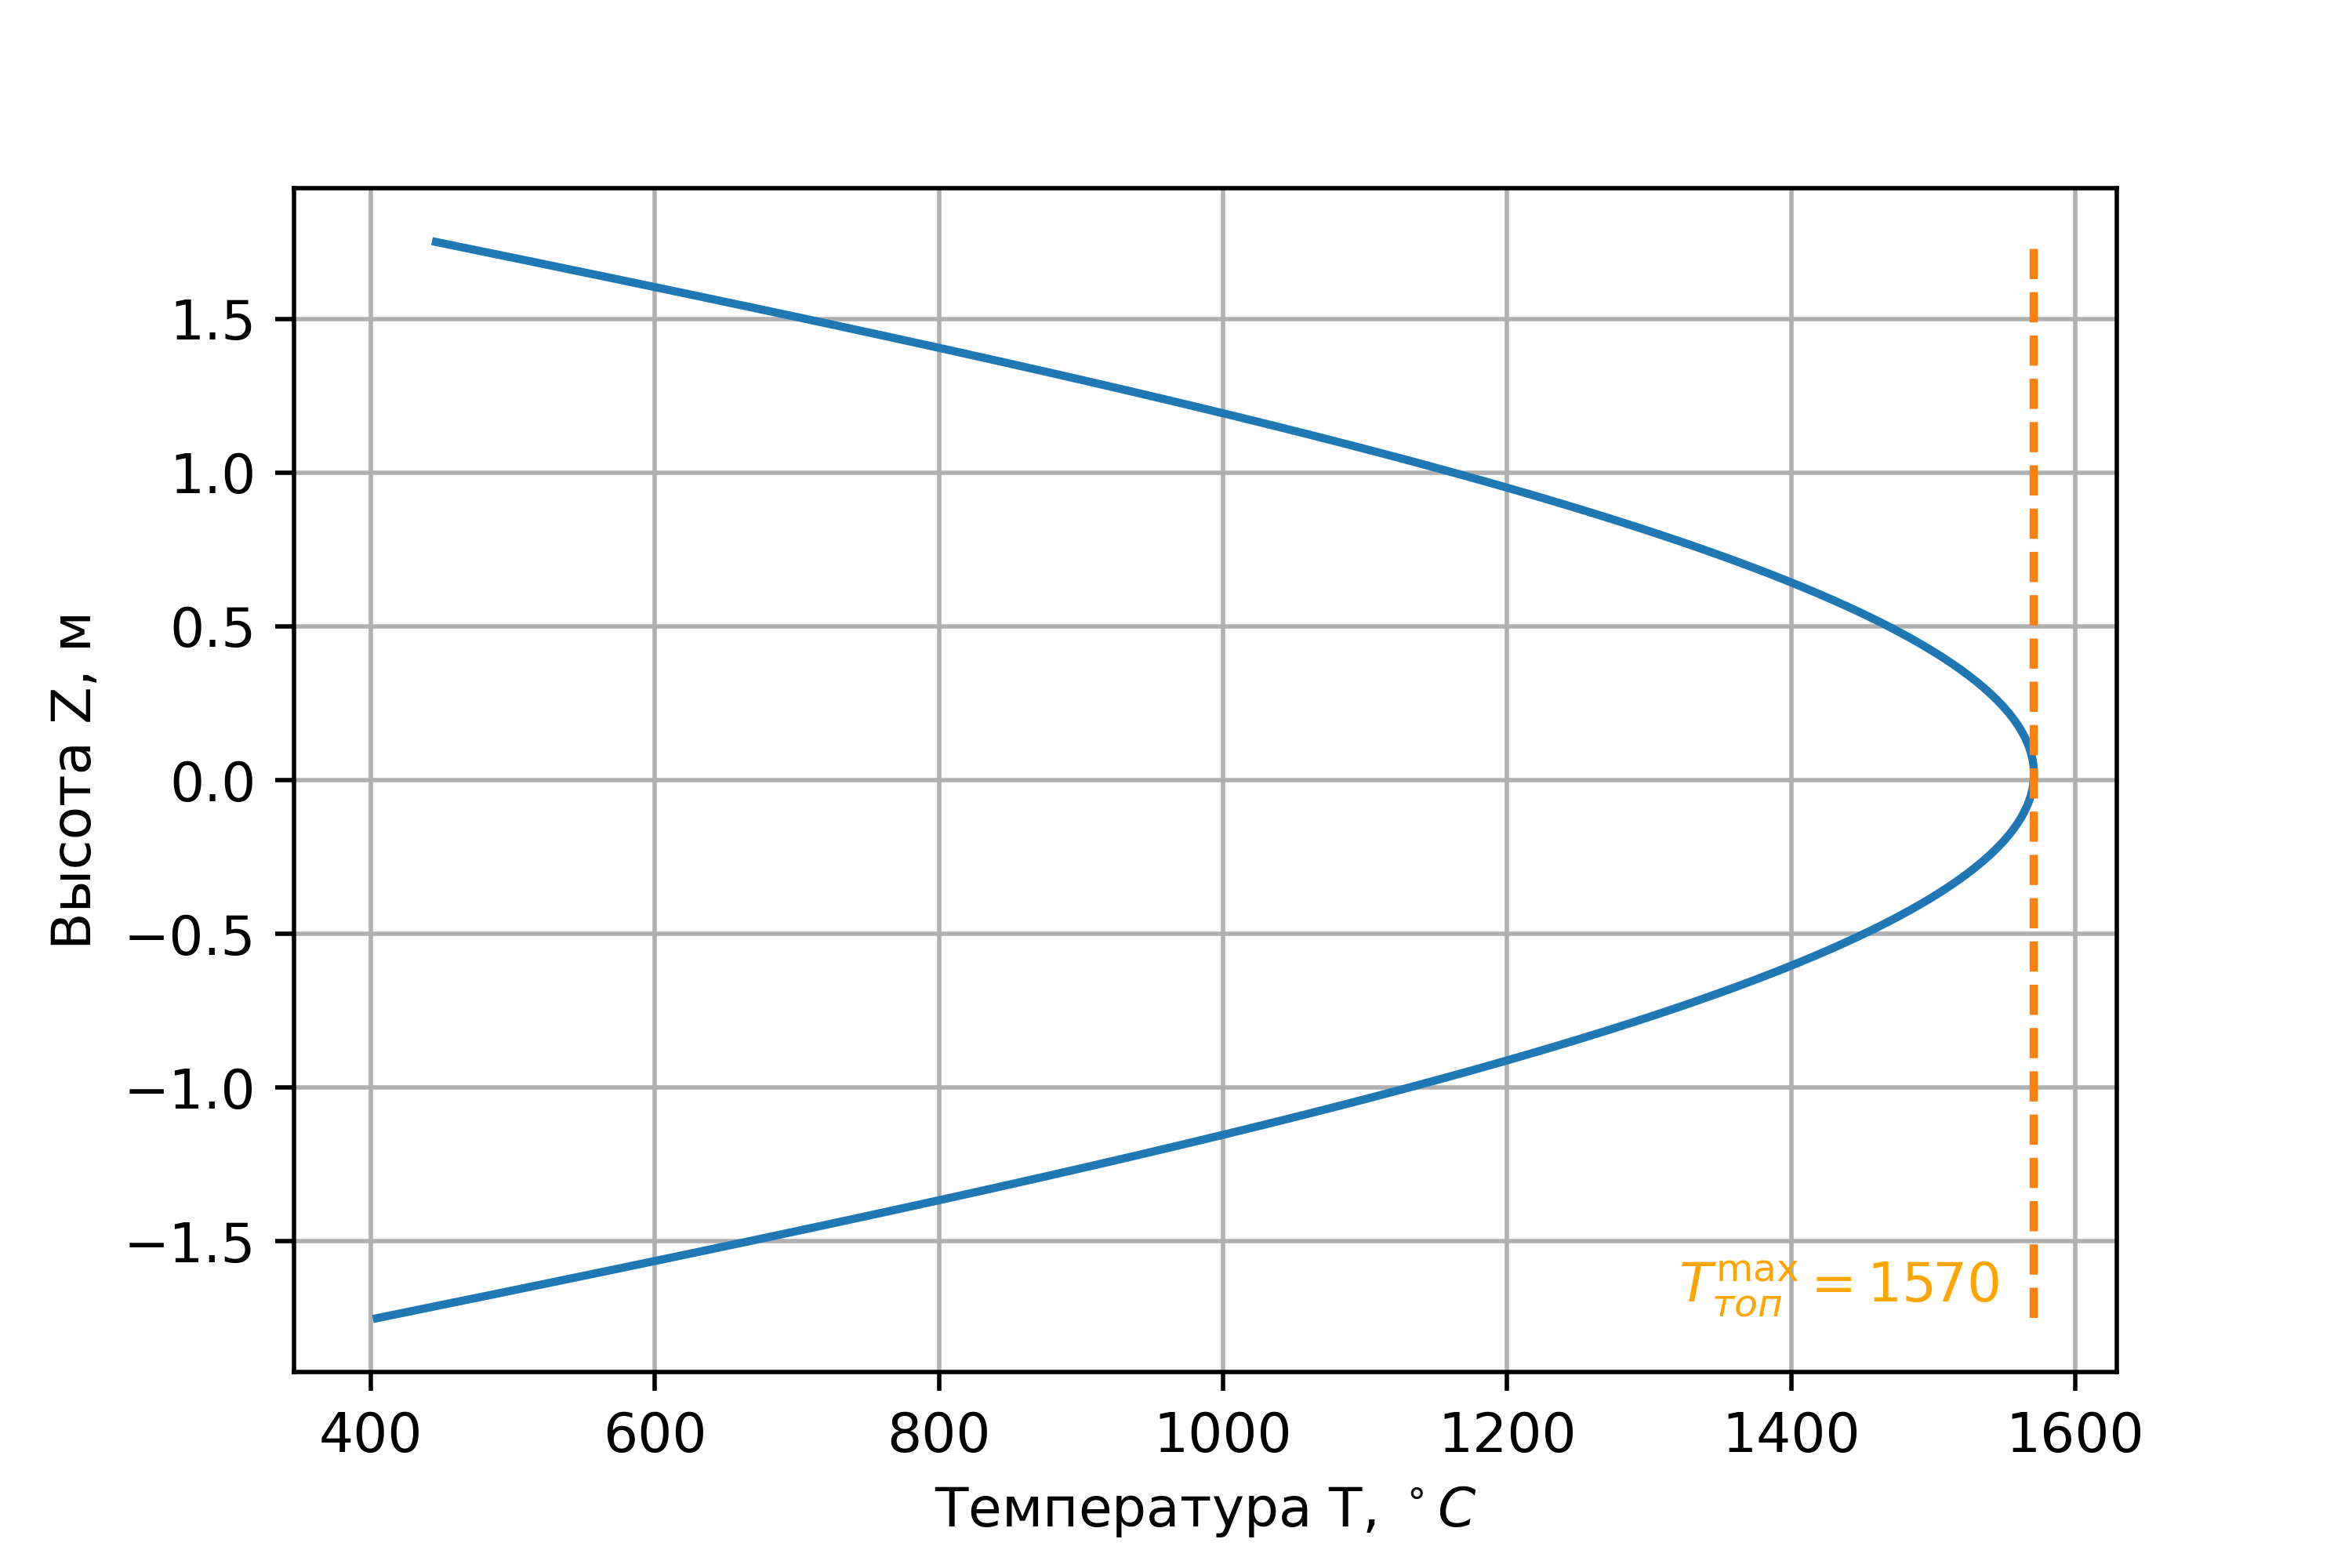
\includegraphics[]{Ttop.png}
		\caption{Изменение температуры топлива по высоте}
		\label{pic:top-referat} % название для ссылок внутри кода
	\end{center}
\end{figure}

\begin{figure}[H]
	\begin{center}
		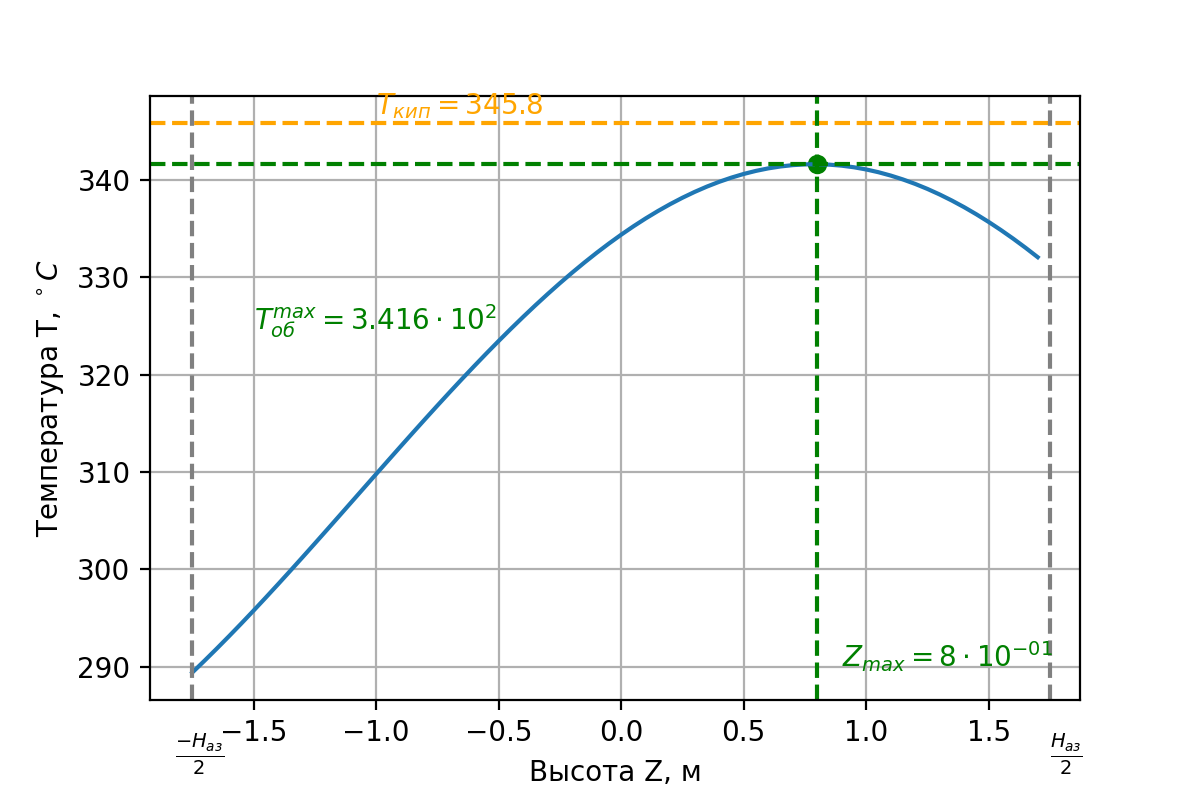
\includegraphics[]{Tob.png}
		\caption{Изменение температуры стенки твэла по высоте}
		\label{pic:Tob-referat} % название для ссылок внутри кода
	\end{center}
\end{figure}

\begin{figure}[H]
	\begin{center}
		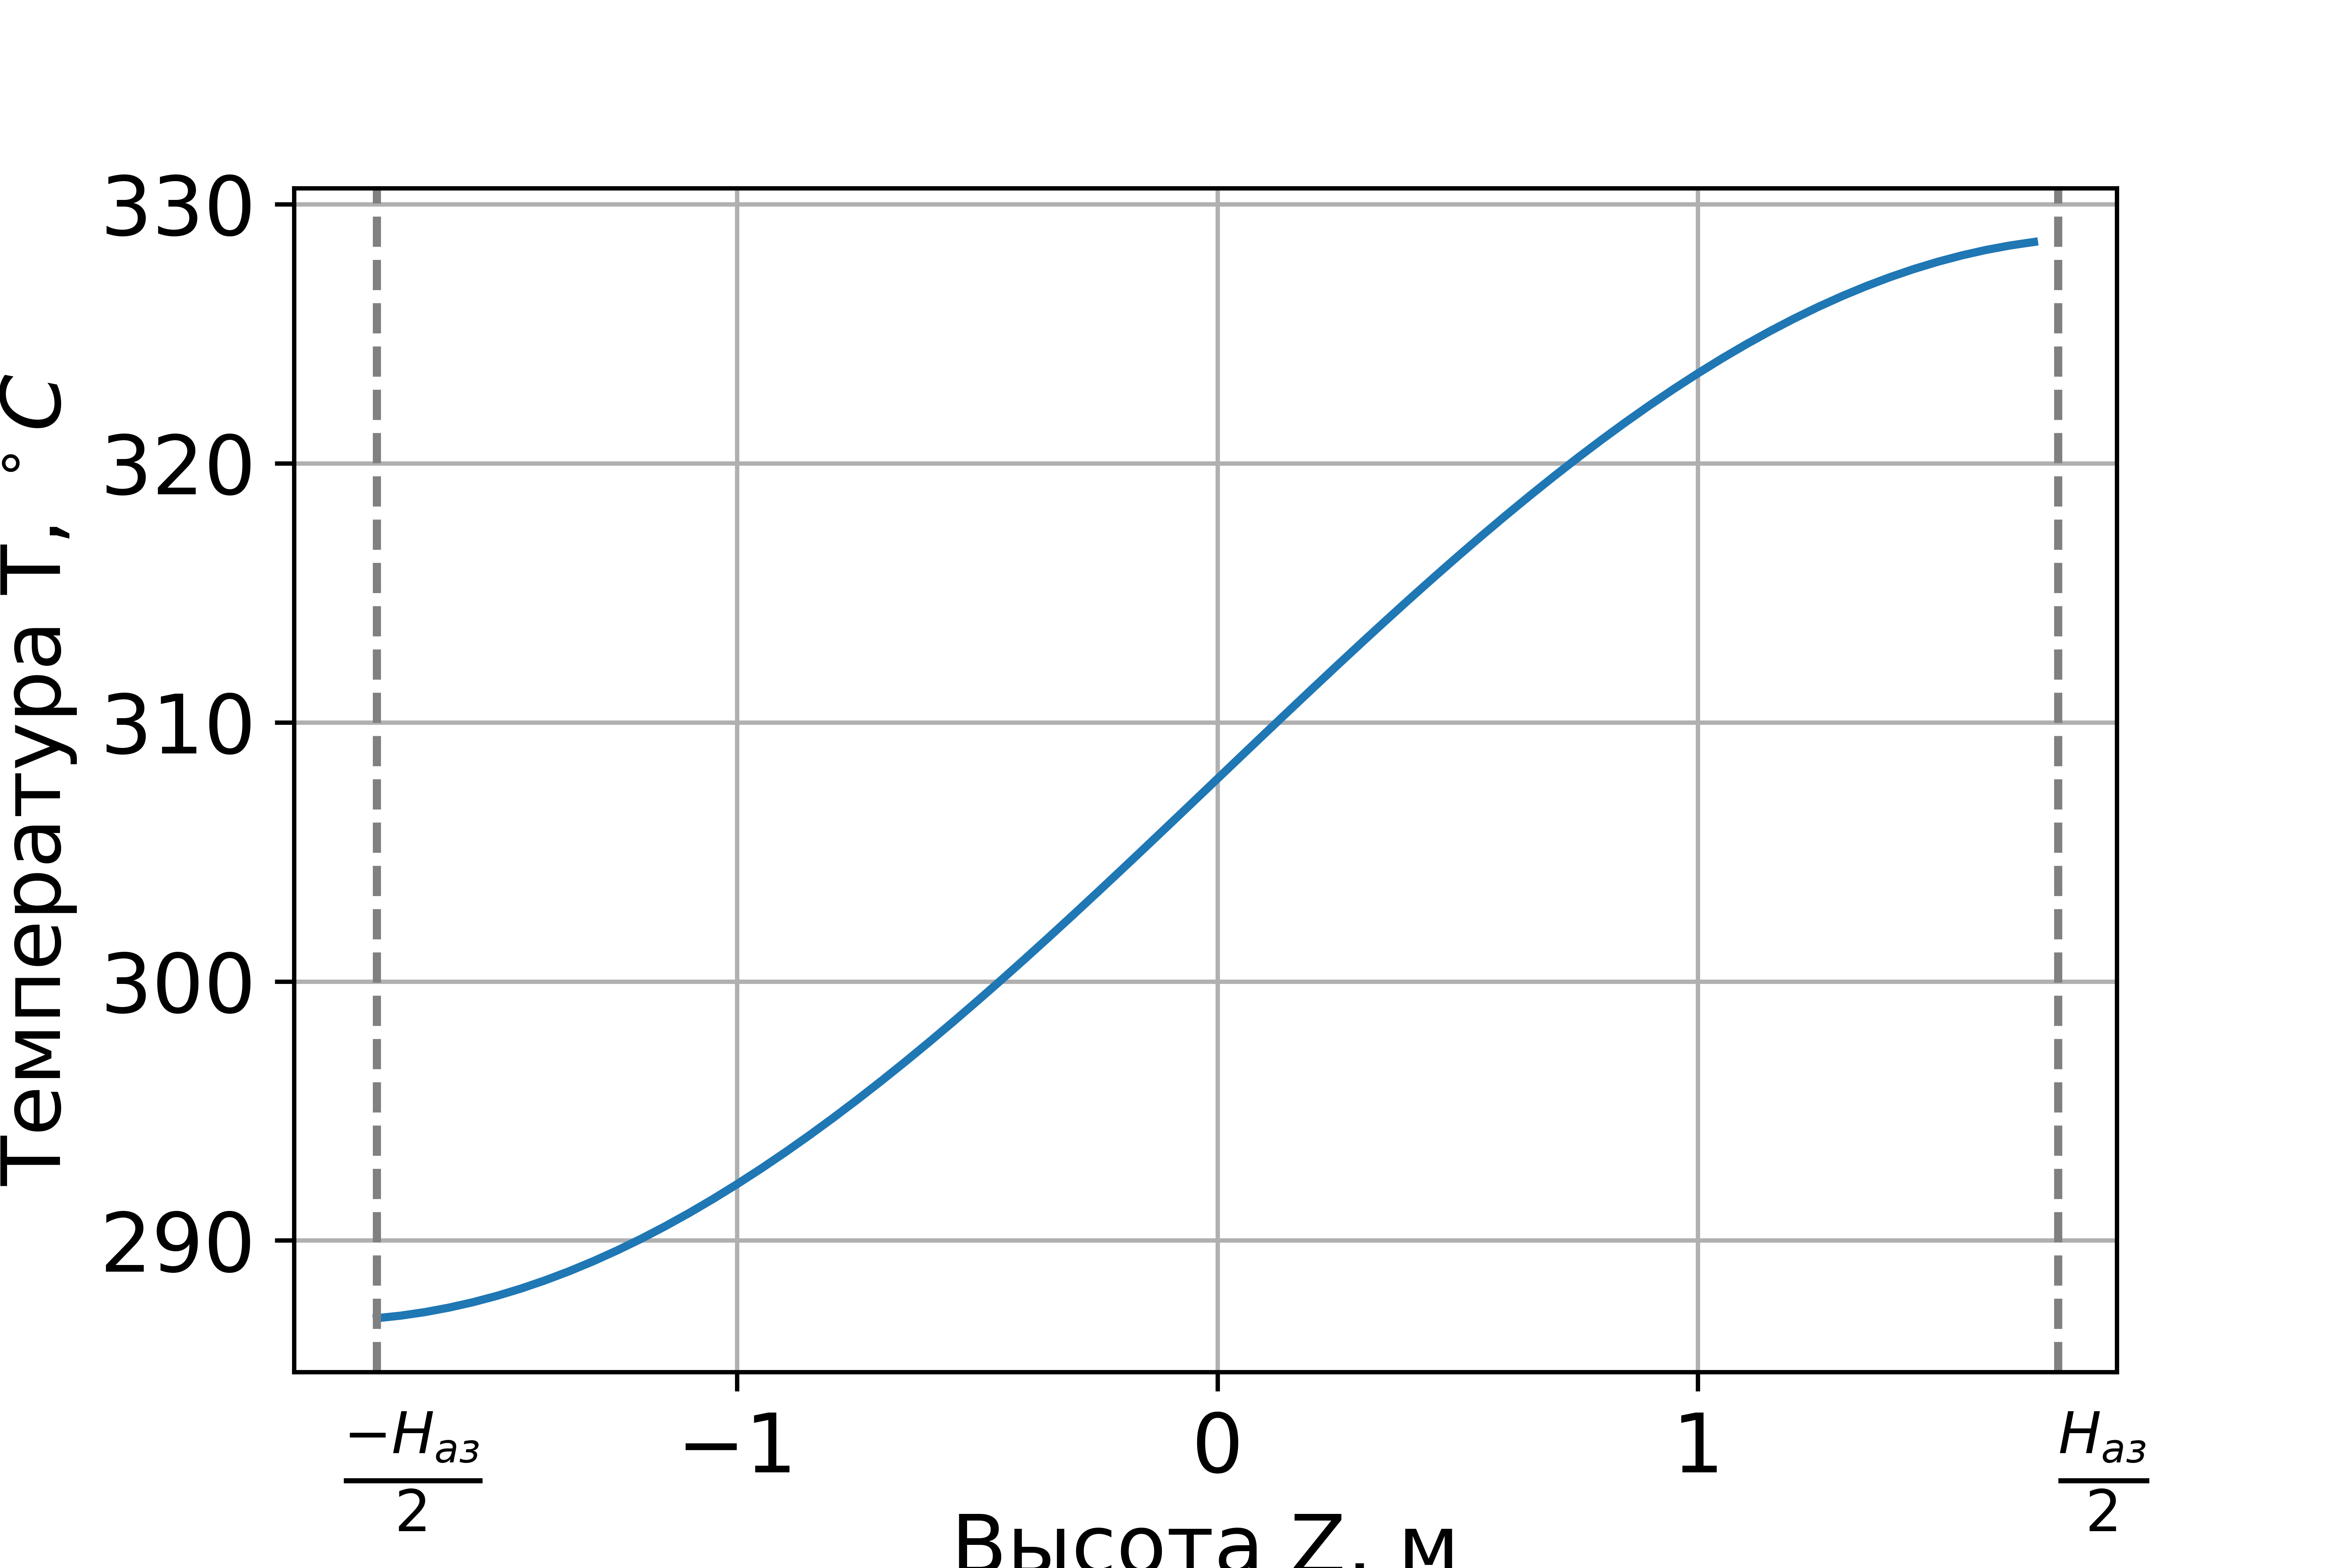
\includegraphics[]{Tz.png}
		\caption{Изменение температуры теплоносителя по высоте}
		\label{pic:TZ-referat} % название для ссылок внутри кода
	\end{center}
\end{figure}

\paragraph{В главе 3} Был произведен нейтронно-физический расчет ячеек активной зоны в приближении бесконечной решетки с помощью програмного комплекса GETERA-93. В рамках расчета бесконечной решетки ТВС без учета выгорания был получен коэффициент $K_{\infty} = 1.38$. Был смоделирован процесс частичных перегрузок для трех циклов выгорания расчетом полиячеек. По результатам расчета было определено оптимальное время цикла прегрузки $T_{\text{цикла}} = 450\ \text{суток}$. По итогам расчета выгорания был jпстроен плутониевый вектор в конце камании, представленый в таблице \ref{tabular:burnup-referat}.

\begin{table}[H]
	\caption{{Характеристики процесса выгорания}}
	\begin{center}
        \begin{tabular}{|c|c|}
        \toprule
         Характеристика & Значение\\ 
         \midrule
         \hline
          $K_\infty$ в начале цикла & $1.1667$\\
         \hline
          Длина цикла, сут & 450 \\
         \hline
          Длина кампании, сут & 1350\\
         \hline
          Выгорание, МВт $\cdot$ сут / кг & $53.541$\\
         \hline
          Годовой расход ТВС, 1 / год & 42.2\\
         \hline
          Плутониевый вектор в конце кампании, \% & \\
         \hline
          $\text{Pu}^{38}$ & 1.97 \\
         \hline
          $\text{Pu}^{39}$ & 55.18 \\
         \hline
          $\text{Pu}^{40}$ & 21.35\\
         \hline
          $\text{Pu}^{41}$ & 15.59 \\
         \hline
          $\text{Pu}^{42}$ & 5.91 \\
         \hline
         Содержание делящегося изотопа (Pu39 + Pu41) в \\ отработавшем топливе, кг/тонна топлива & 14.87\\
         \hline
         Содержание делящегося изотопа (U235)\\ в отработавшем топливе, кг/тонна топлива & 11.4 \\
         \hline
         Загрузка делящихся нуклидов, кг/тонна топлива & 47 \\
         \bottomrule
		\end{tabular}
		\label{tabular:burnup-referat}
	\end{center}
\end{table}

\paragraph*{В главе 3} был произведен анализ и расчет програмным комплексом ТРЕТОН следующих режимов работы реактора:
\begin{itemize}
    \item номинальный режим
    \item режим на повышенном уровне мощности
    \item режим на пониженном уровне мощности при отключении одного ГЦН
    \item режим на пониженном уровне мощности при отключении двух ГЦН
\end{itemize}

Для номинального режима работы было проведено сравнение расчетов температур теплоносителя, топлива и оболочки с теплофизическим расчетом, для теплоносителя и оболочки температуры совпадают в рамках поггрешности задания среднего коэффициента теплоемкости, для топлива различие обусловлено особенностей задания характеристик материалов входящих в состав топилва.

\begin{figure}[H]
	\begin{center}
		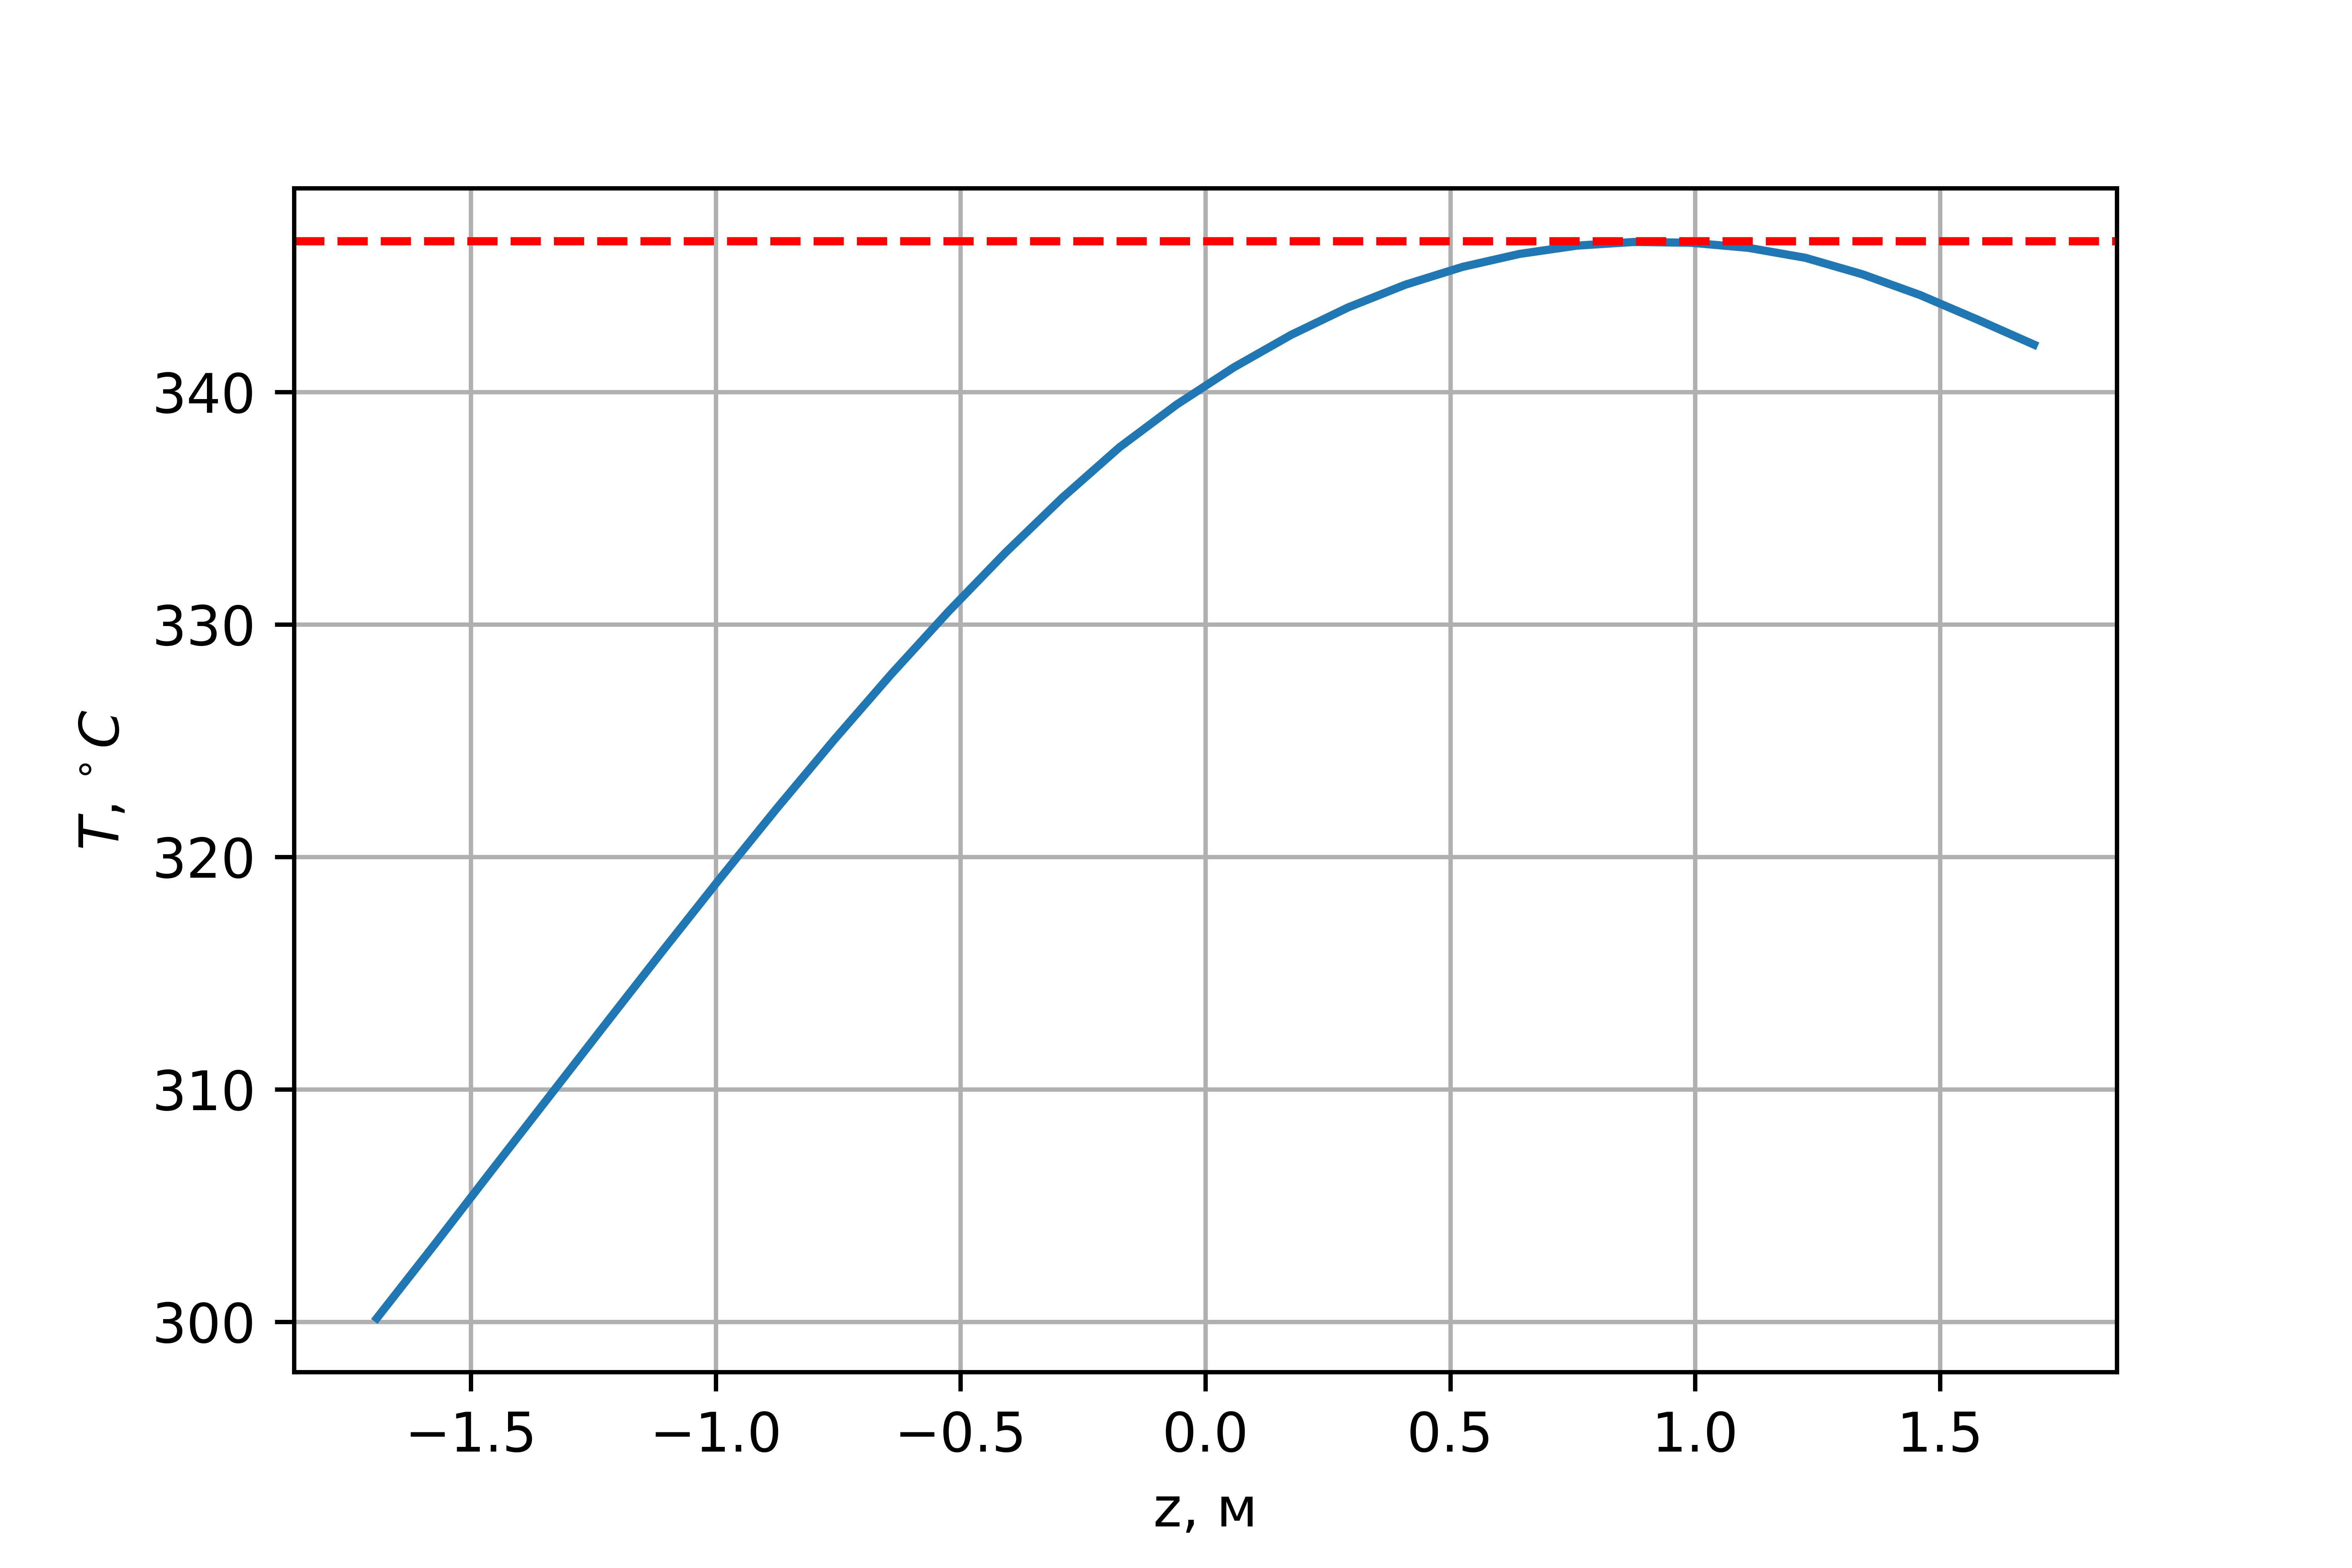
\includegraphics{treton_nominal_obl_naruj_max.png}
		\caption{Распределение температуры внешней оболочки по высоте для кассеты с максимальной температурой на выходе из АЗ}
	\end{center}
\end{figure}

\begin{figure}[H]
	\begin{center}
		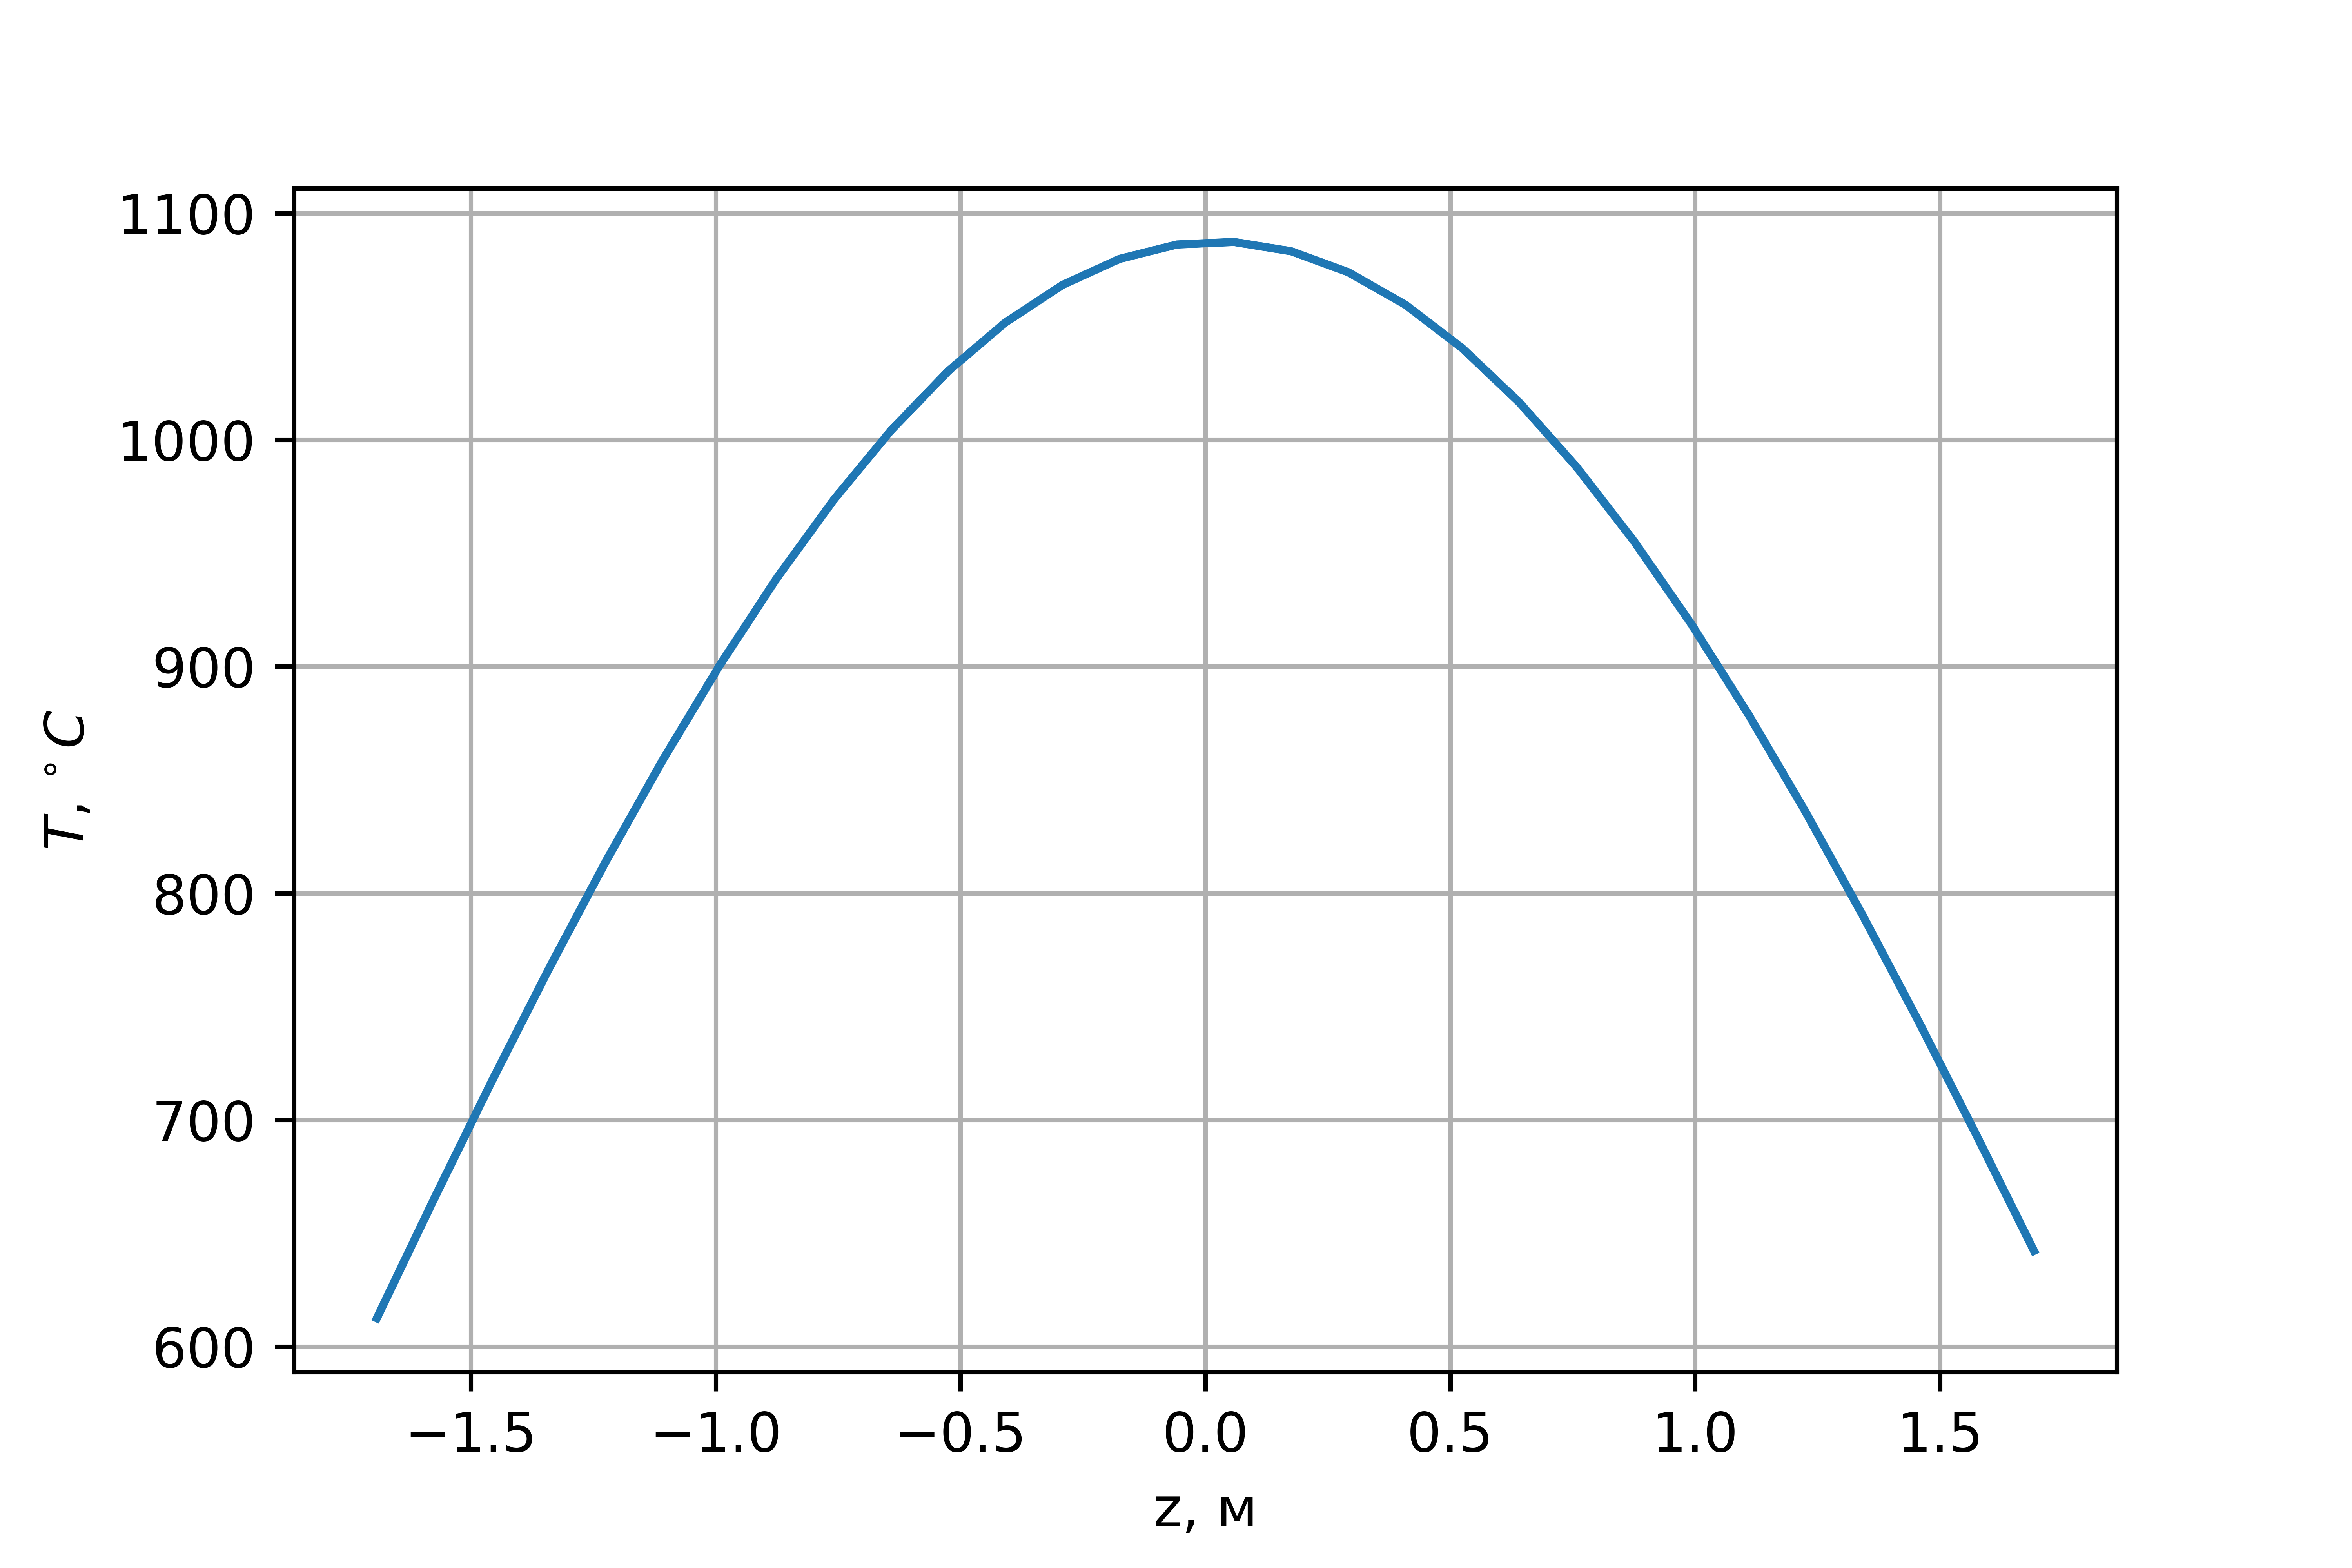
\includegraphics{treton_nominal_t_fuel_max.png}
		\caption{Распределение температуры топлива по высоте АЗ для кассеты с максимальной температурой топлива в центре АЗ}
	\end{center}
\end{figure}

\begin{figure}[H]
	\begin{center}
		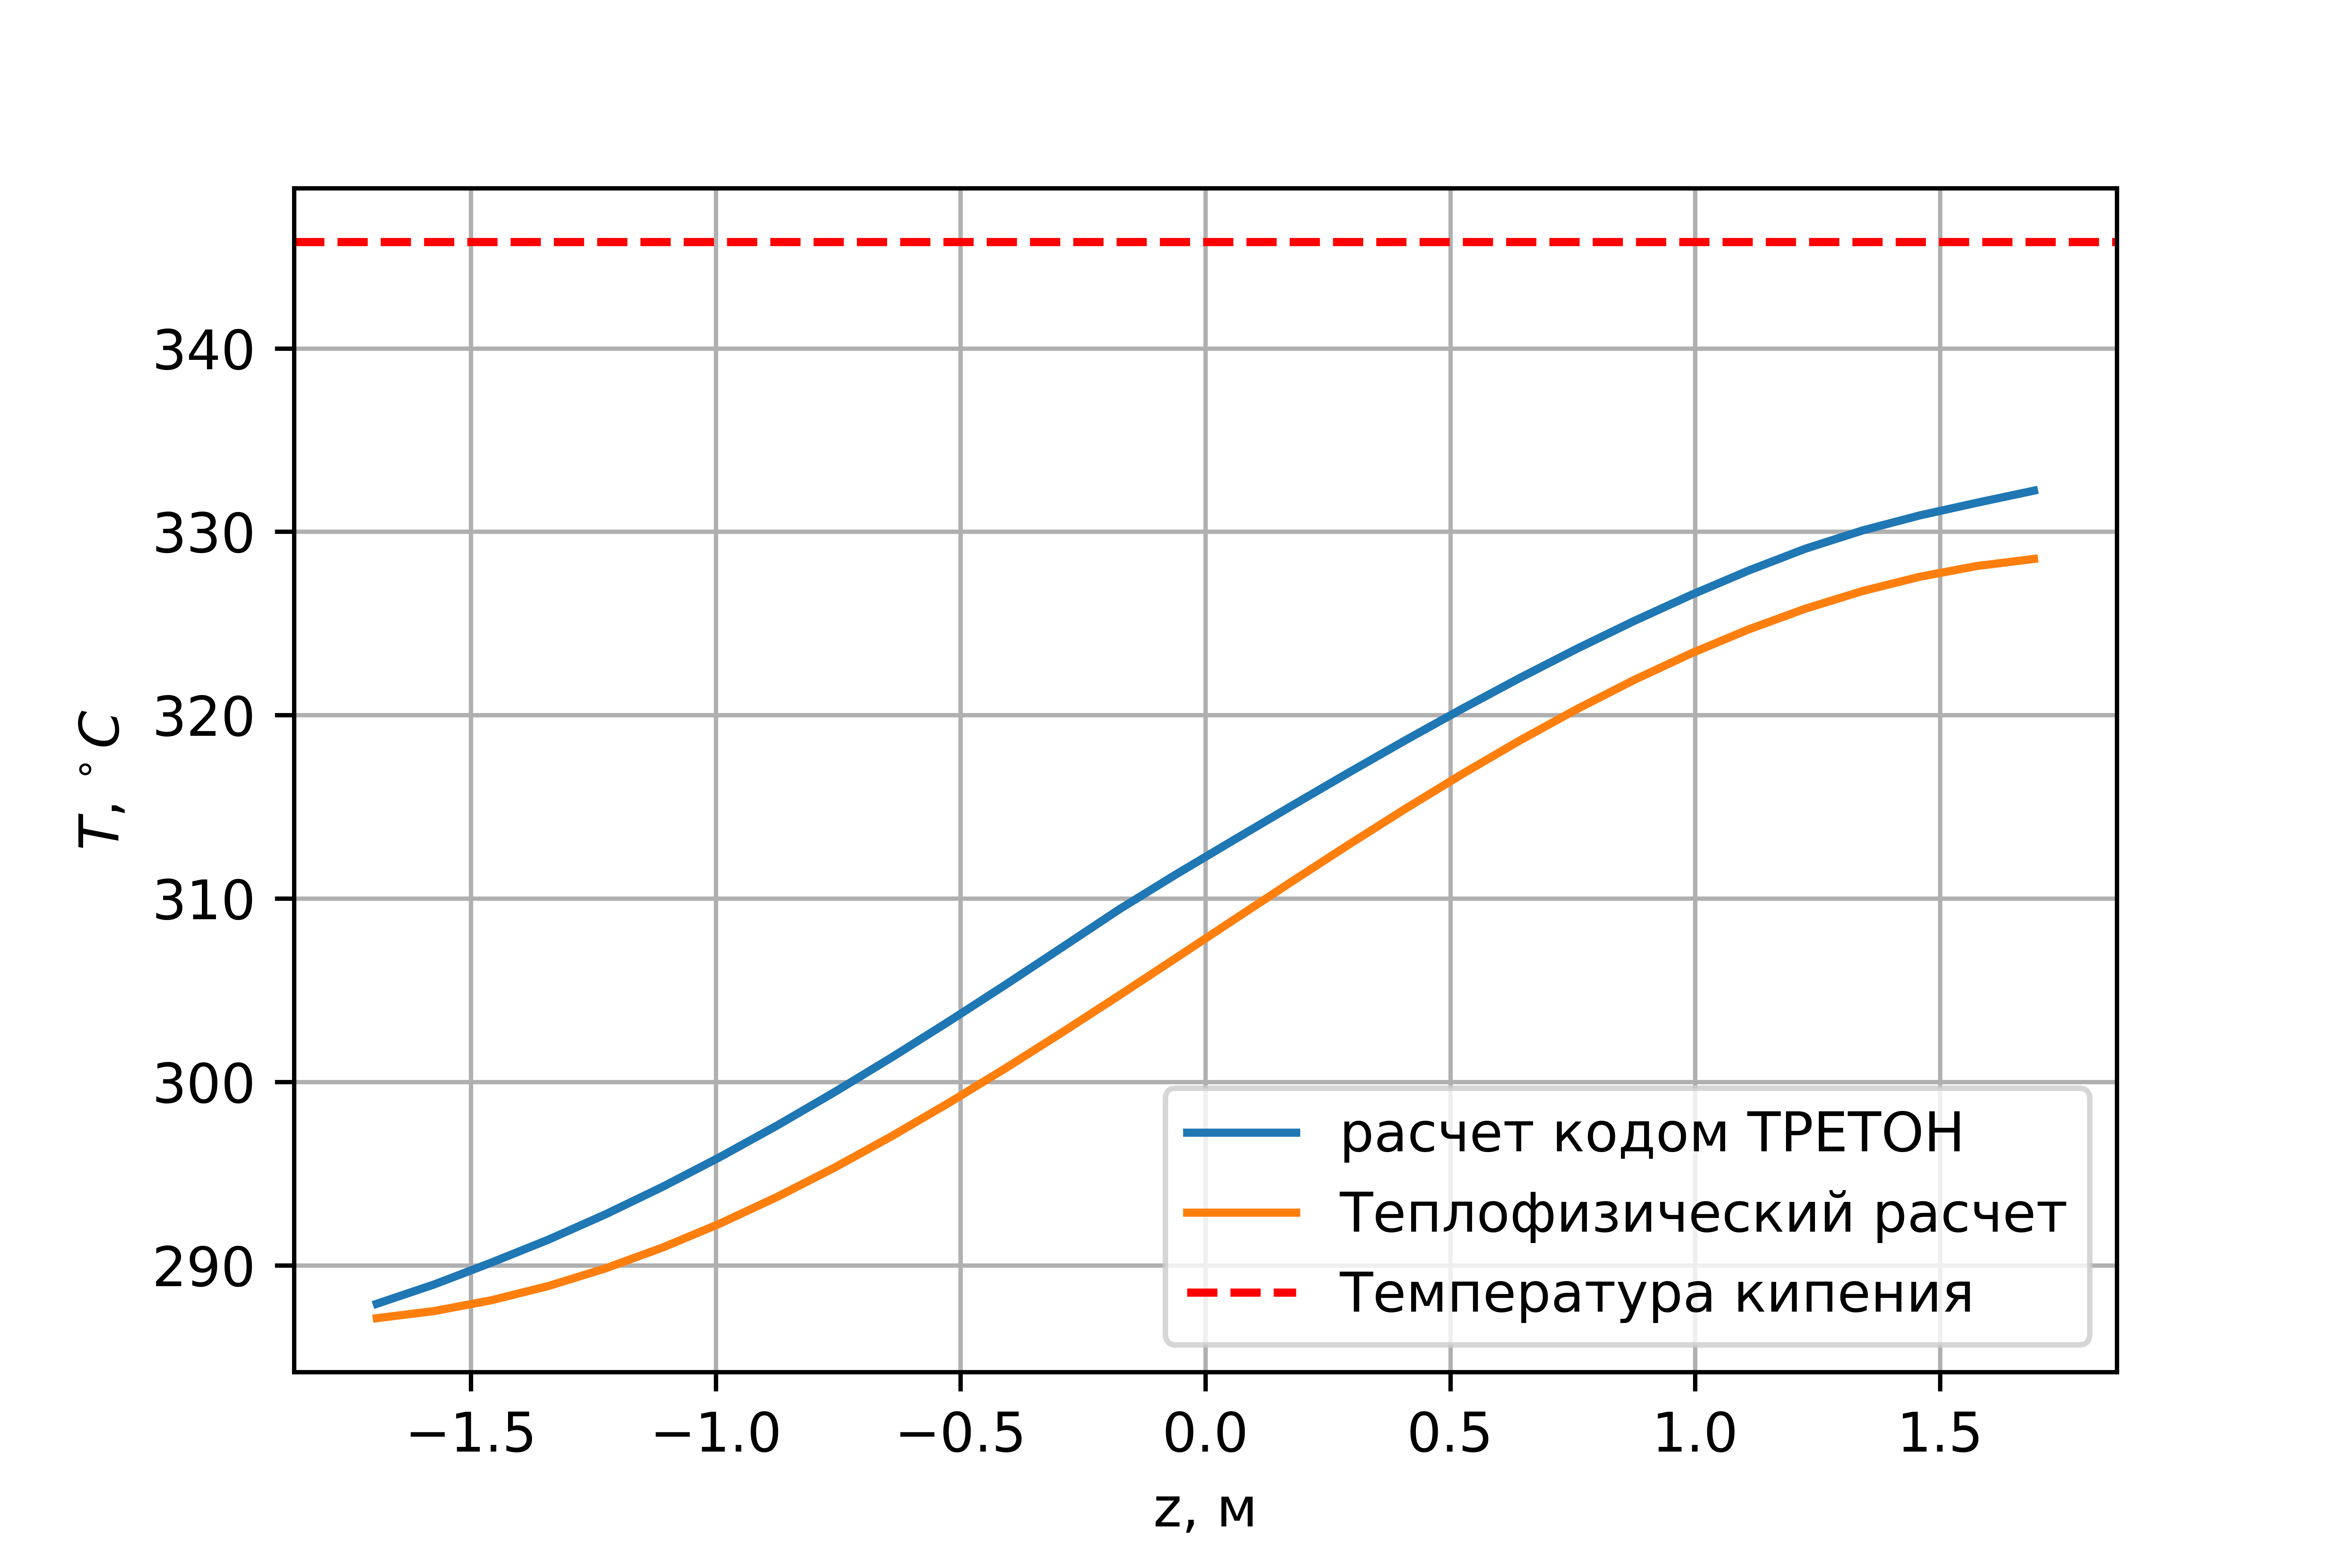
\includegraphics{treton_nominal_t_z.png}
		\caption{Распределение температуры теплоносителя по высоте}
	\end{center}
\end{figure}

Для режима повышенной мощности была определена оптимальная мощность, при которой эффект пристеночного кипения не существенен. Были рассмотрены мощности 105\%, 110\%, 115\% от номинальной. По результатам сравнения оптимальной была выбрана мощность 105\% ввиду превышения для оболочки температуры кипения теплоносителя не более чем на 3 градуса. 

\begin{table}[H]
    \caption{Максимальные температуры теплоносителя, топлива и оболочки твэлов при работе РУ на номинальной и повышенной мощности}
    \begin{center}
        \begin{tabular}{|l|c|c|c|c|}
        \toprule
        Тепловая мощность, МВт & 2903 & 3048.8 & 3194 & 3339.2 \\
        \midrule
        \hline
        Максимальная температура теплоносителя, $\circ C$ & 332.5 & 333.9 & 334.9 & 336.3  \\ 
        \hline
        Запас до кипения теплоносителя, $\circ C$ & 13.9 & 12.6 & 11.6 &  10.17 \\
        \hline
        Максимальная температура топлива, $\circ C$ & 1452 & 1465 & 1501.8 & 1538.4  \\
        \hline
        Максимальная температура внешней оболочки & 346.46 & 347.9 & 349  & 349.4 \\
        \hline
        Максимальная температура внутренней оболочки & 381.3 & 383 & 385.9 & 389.7 \\
        \hline
        Разность температуры кипения теплоносителя и температуры внешней оболочки & 0.04 & -1.4 & -2.5 & -2.9 \\
        \bottomrule
        \end{tabular}
    \end{center}
\end{table}

По результатам расчета режима повышенной мощности были получены максимальные значения топлива, оболочек и теплоносителя 1502, 347.9, 334, $^\circ C$ соответственно. Полученные результаты не превышают температур насыщения, для оболочки превышение температуры кипения теплоносителя несущественно. Из чего можно сделать вывод о возможности эксплуатации ВВЭР-1000 на мощности 105\% от номинальной.

Для режима с отключением одного из гцн были также расчитаны максимальные температуры топлива, оболочек и теплоносителя 1202, 335, 324.5 $^\circ C$ соответственно. Также получены распределения температур по всем твелам, на которых наблюдается перекос в захоложенной области отключение ГЦН. По итогу расчета омжно сделать вывод о возможности использования реактора ВВЭР-1000 при неработающем одном насосе, так как превышений темпераутр насыщения не происходит.

\begin{figure}[H]
	\begin{center}
		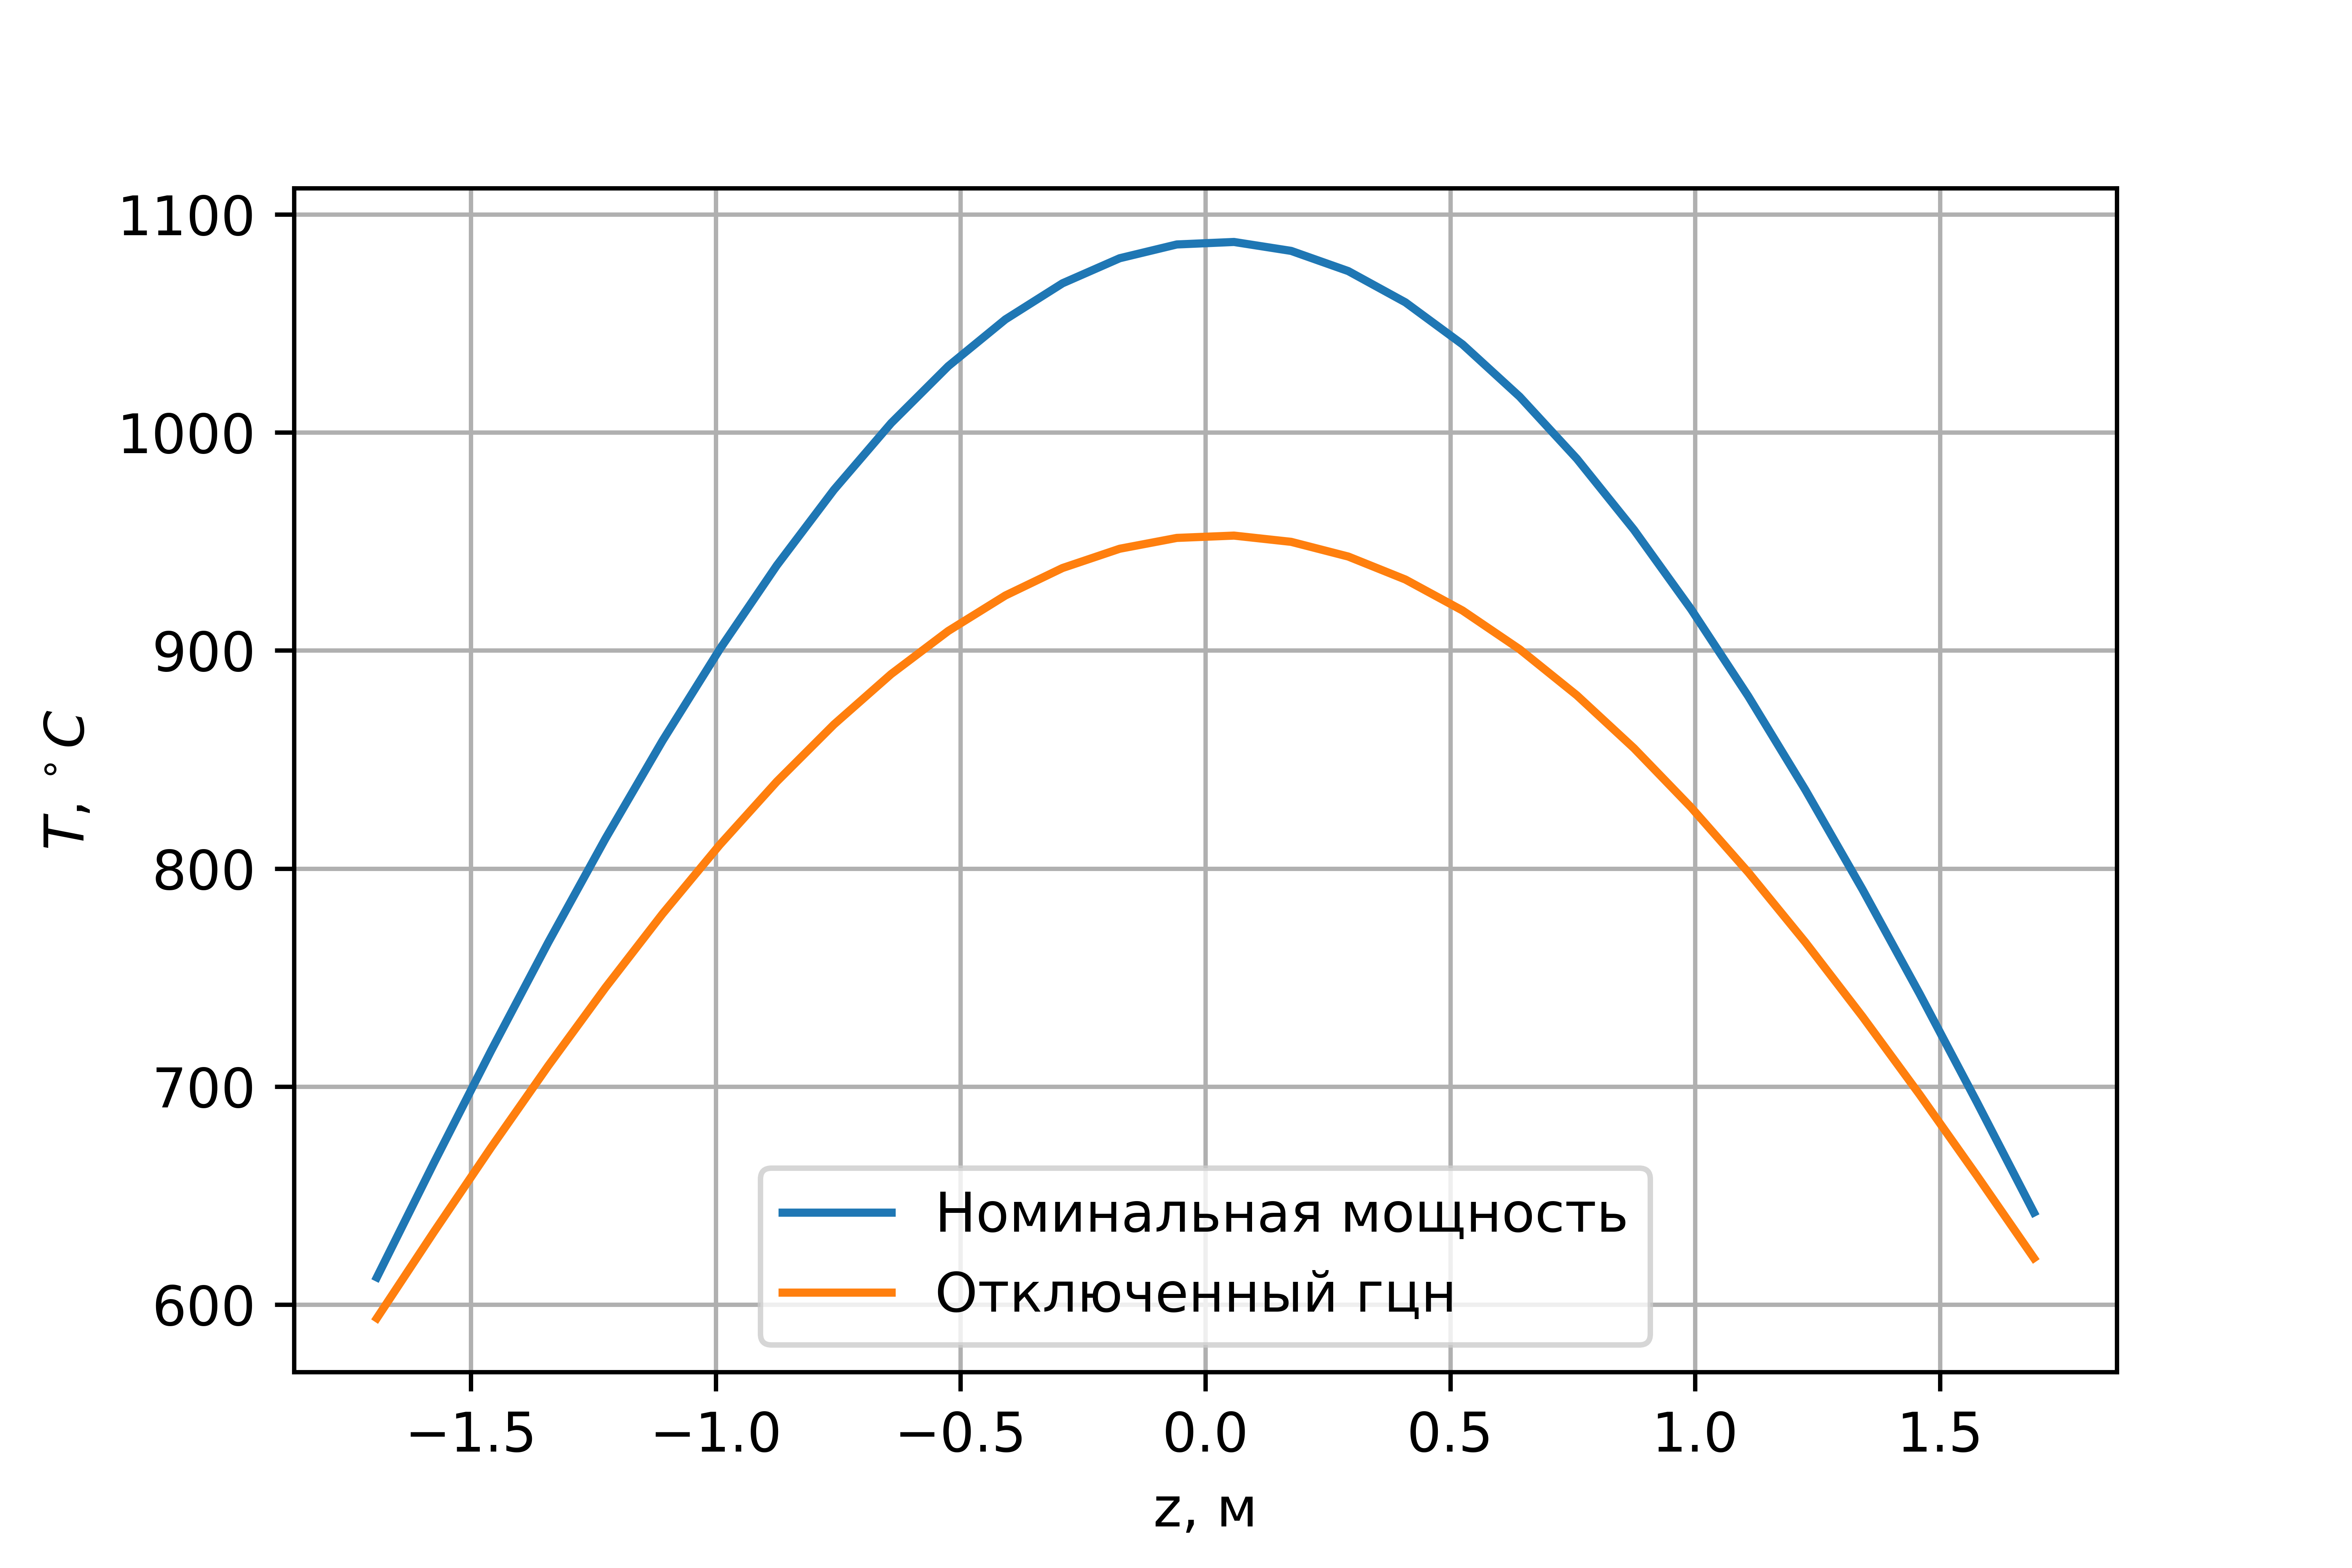
\includegraphics{treton_t_fuel_one_gcn_compare.png}
		\caption{Распределение температуры топлива по высоте АЗ}
	\end{center}
\end{figure}

\begin{figure}[H]
	\begin{center}
		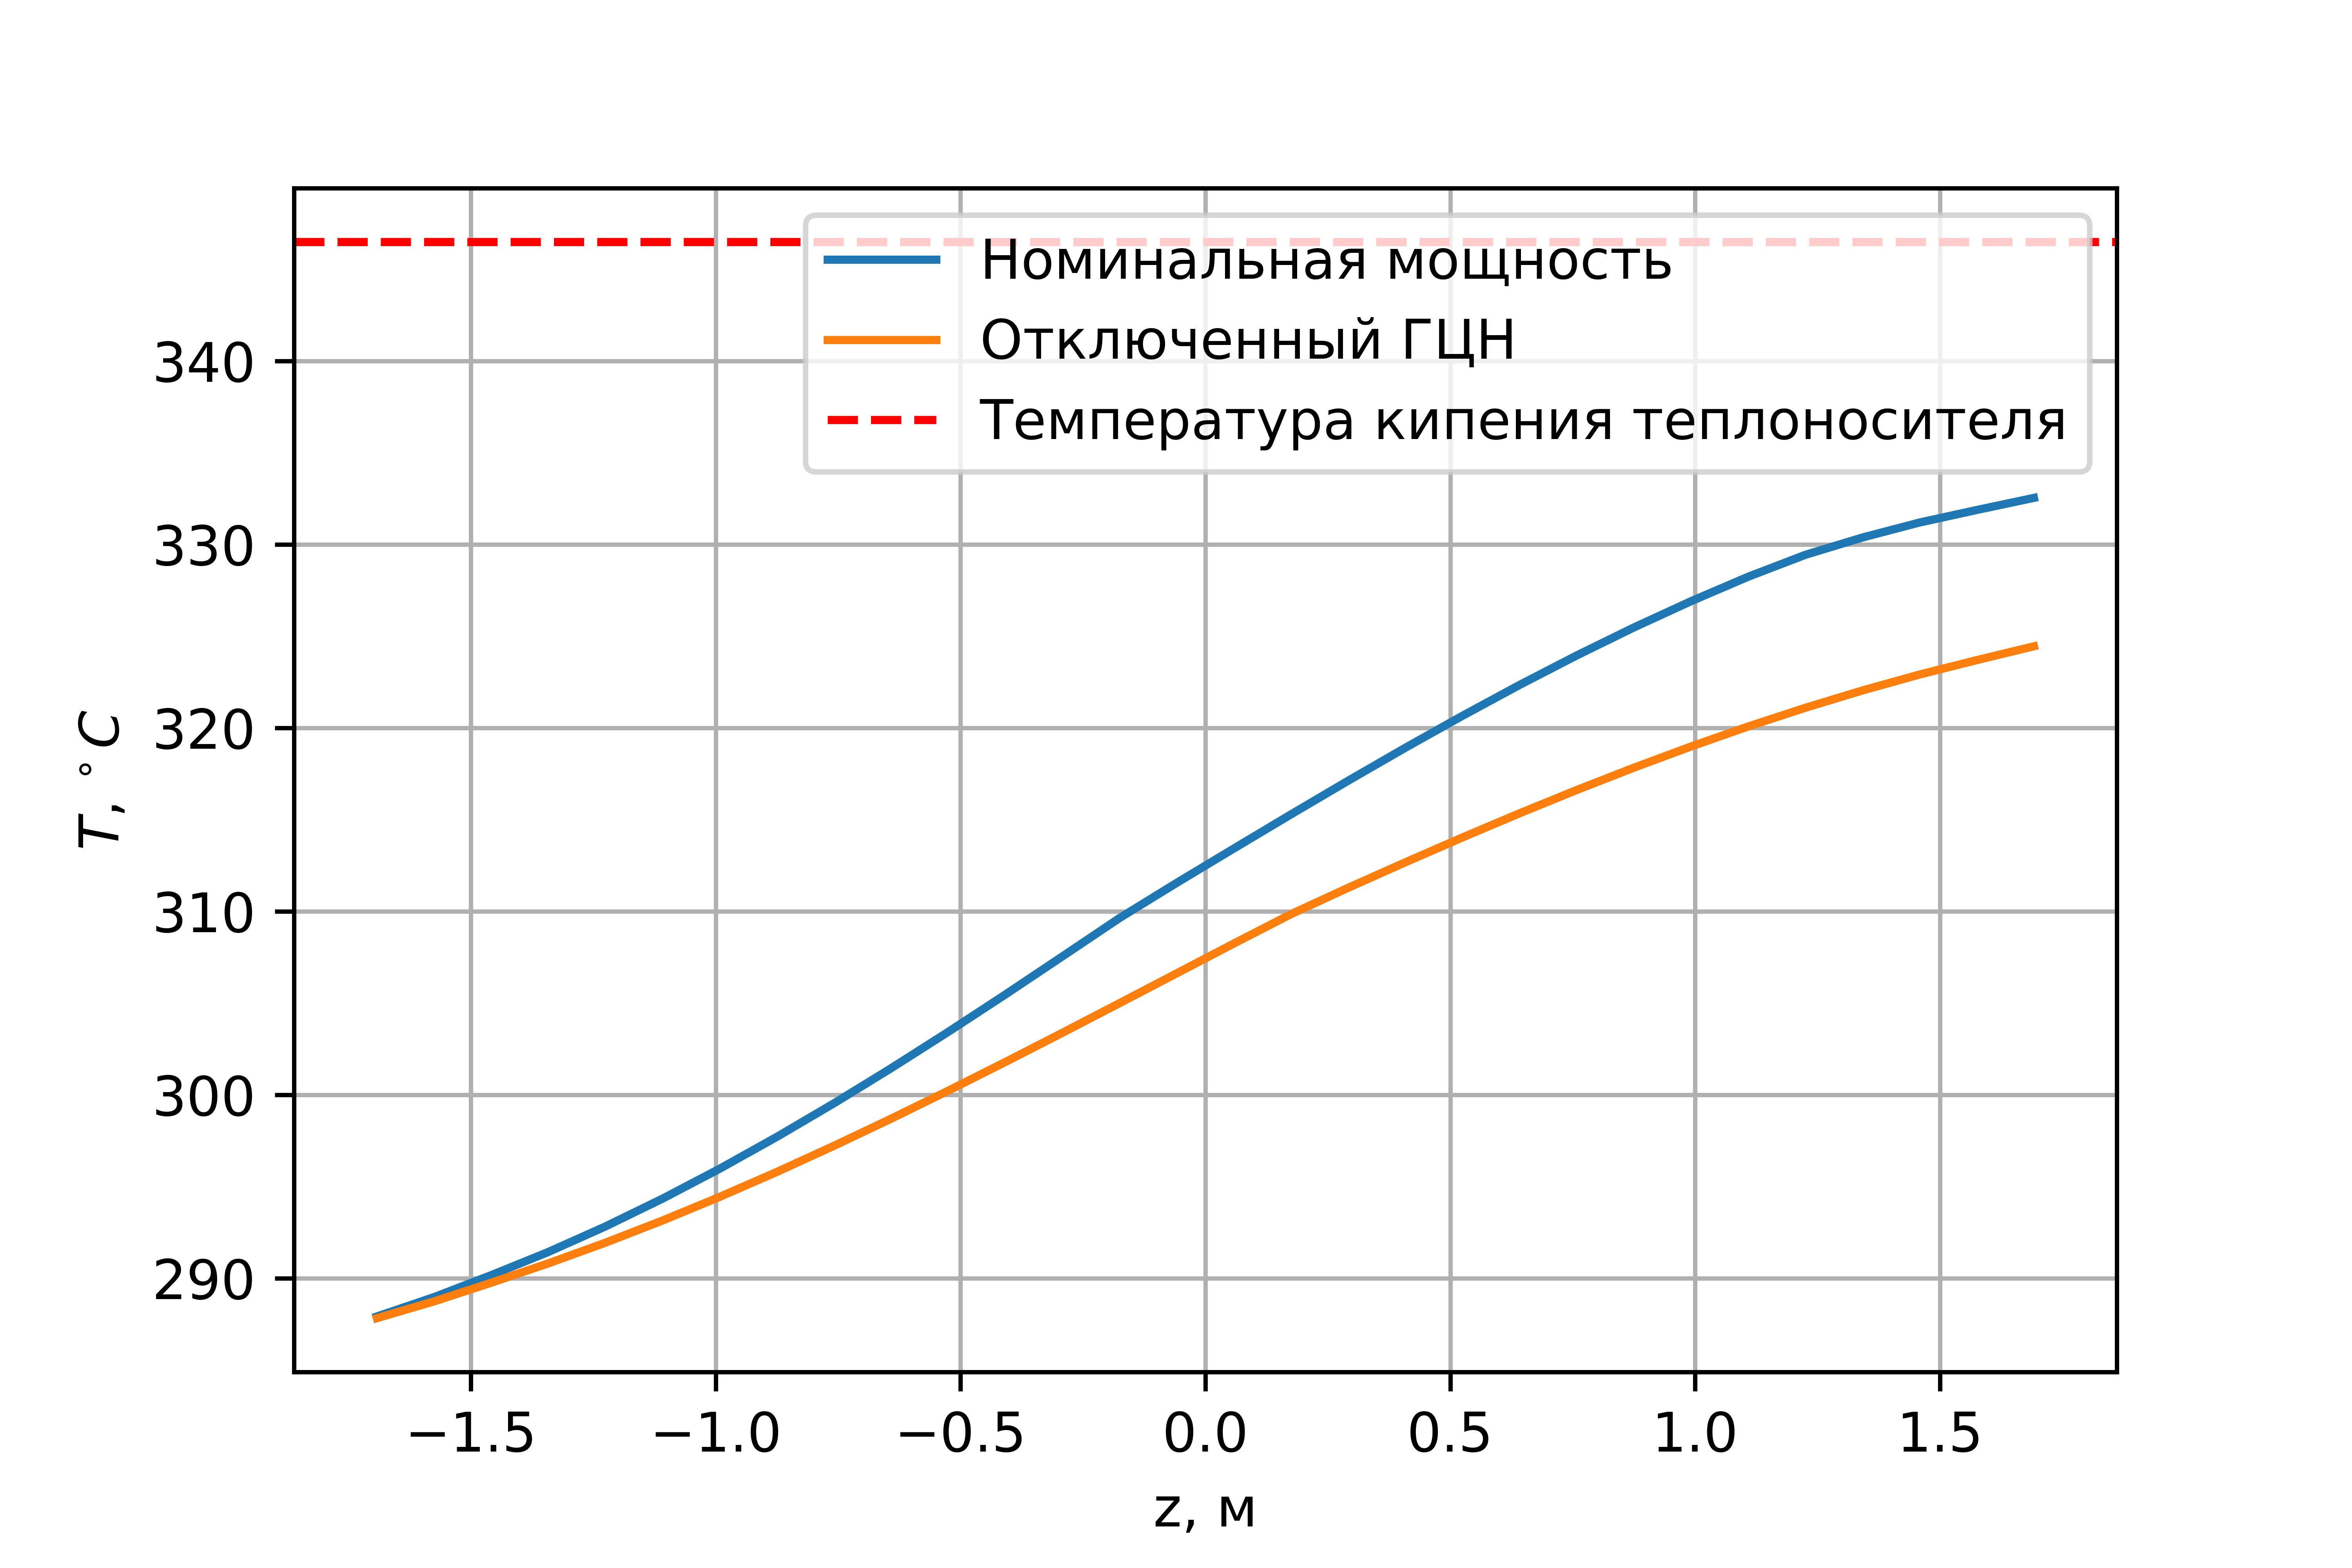
\includegraphics{treton_t_tepl_one_gcn_compare.png}
		\caption{Распределение температуры теплоносителя по высоте АЗ}
	\end{center}
\end{figure}

\begin{figure}[H]
	\begin{center}
		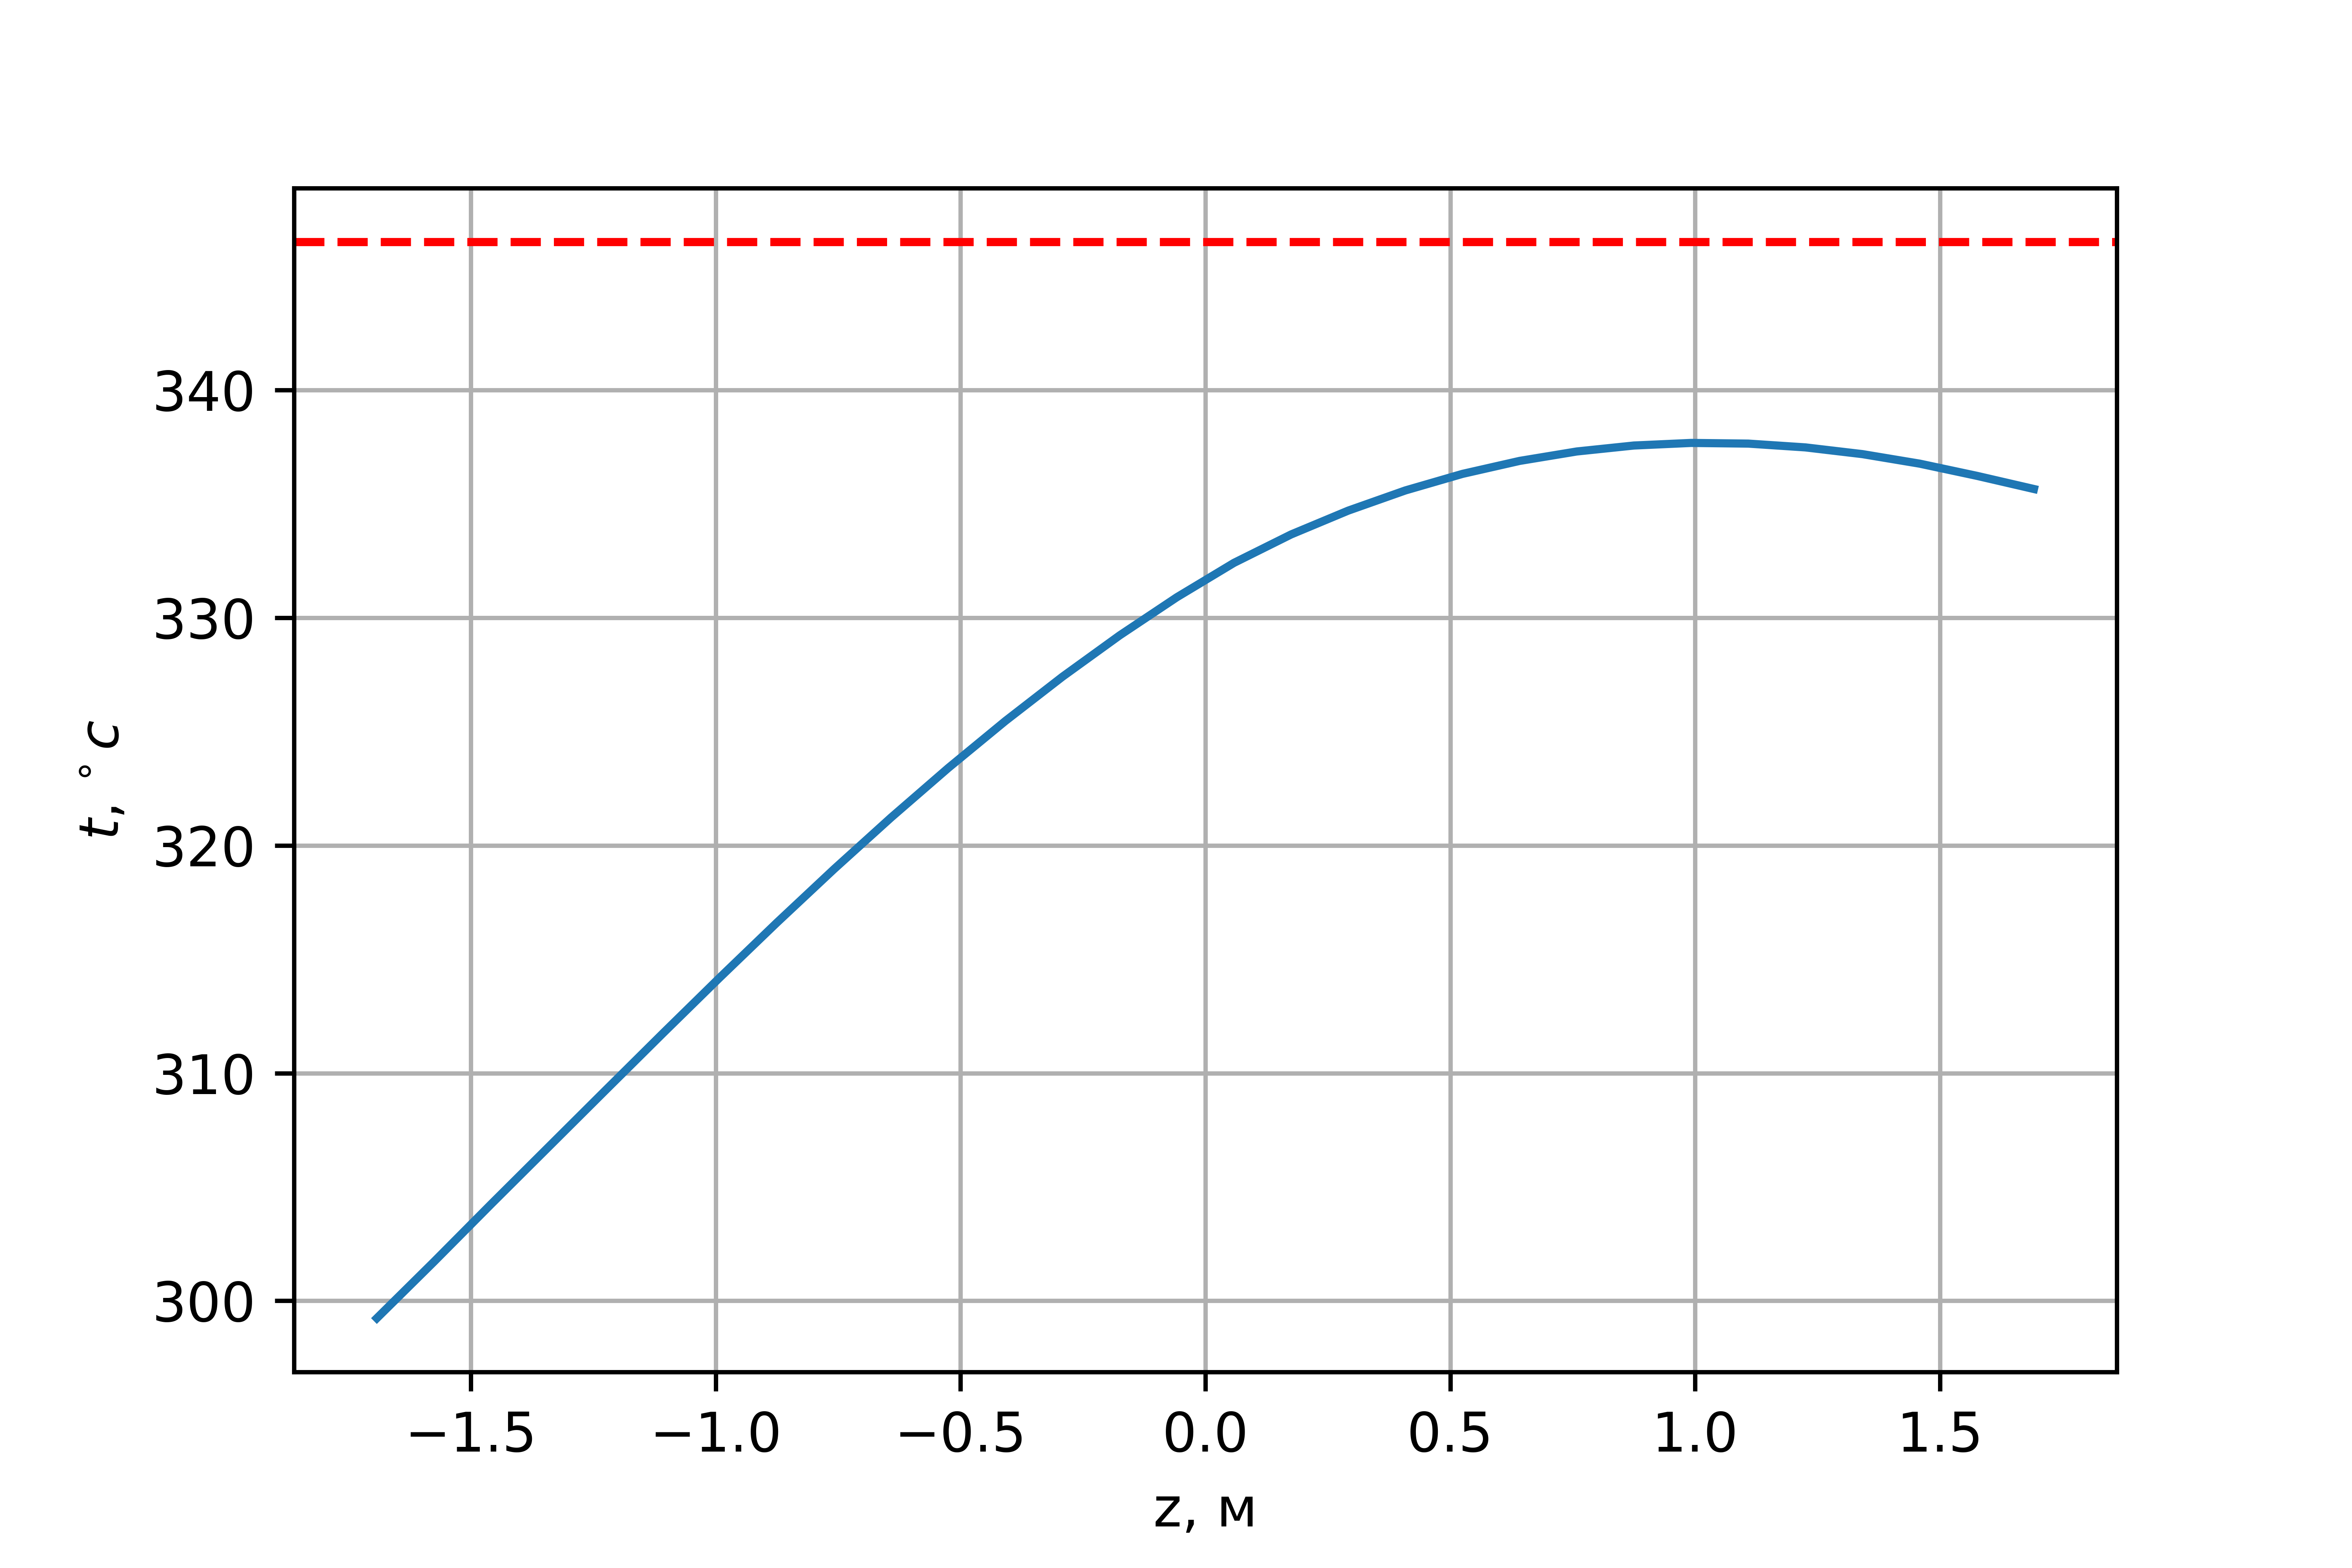
\includegraphics{treton_one_gcn_obl_naruj_max.png}
		\caption{Распределение температуры наруженй оболочки твэлов по высоте для кассеты с максимальной температурой теплоносителя}
	\end{center}
\end{figure}

Для режима с отключением двух стоящх друг на против друга гцн были расчитаны максимальные температуры топлива, оболочек и теплоносителя 1068, 330, 321 $^\circ C$ соотвенно. Также получены распределения температур по всем твелам, на которых наблюдаются установившиеся две зоны температур в следствие захолаживания топилва. По итогу расчета можно сделать вывод о возможности использования реактора ВВЭР-1000 при неработающих двух гцн на пониженной мощности, так как превышений температур насыщения не происходит.


\subsection*{ОСНОВНЫЕ ВЫВОДЫ}
\begin{enumerate}
    \item Для расчета теплогидравлических параметров ВВЭР-1000 с бесчехловыми твс применима модель анизотропного пористого тела и расчет с помощью програмного комплекса ТРЕТОН сходится с теплофизическим теоритическим расчетом в пределах погрешности
    \item При повышении мощности ВВЭР-1000 на 5\% существенных превышений температур насыщения не наблюдается и установка работоспособна в таком режиме 
    \item РУ может работать при отключении одного либо двух стоящих друг на против друга ГЦН, температуры насыщения в таких режимах не превышаются
\end{enumerate}



\noindent КЛЮЧЕВЫЕ СЛОВА: ВВЭР-1000, ТРЕТОН, повышенная мощность, отключение гцн.
